\section{Margaret (Dooley) (Simonds) Fernald}\label{per:Margaret3Dooley}

\begin{figure}[htbp]
	\centering
	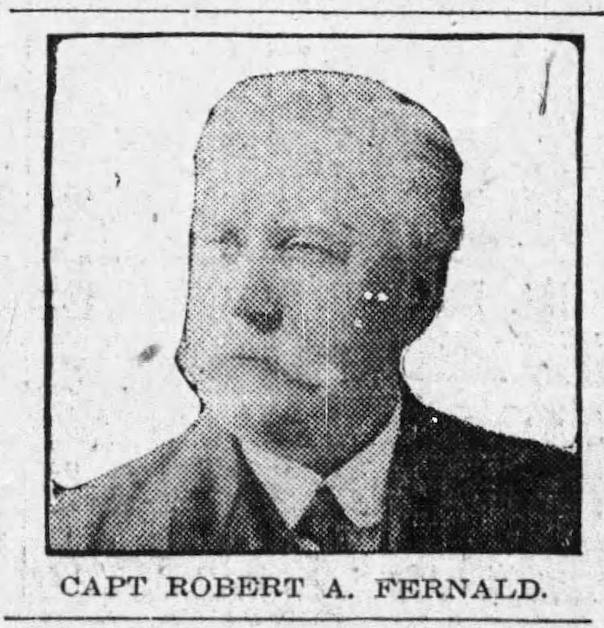
\includegraphics[width=1.5in]{fernald}
	\caption{Captain Robert A.\ Fernald.\index{Fernald!Robert}}
	\label{fig:RobertFernald}
\end{figure}

\MainPerson{Margaret\textsuperscript{3} Dooley}\index{Dooley!Margaret\textsuperscript{3}|bb}\index{Simonds!Margaret\textsuperscript{3} (Dooley)}\index{Fernald!Margaret\textsuperscript{3} (Dooley) (Simonds)} (\Lineage{2}{Abigail}, \Lineage{1}{William}) was born in Watergrasshill, County Cork, Ireland,\index{Ireland!Watergrasshill, County Cork} 27 December 1840.\cite{Margaret3DooleyBaptism:2} She died in Boston, Suffolk County, Massachusetts,\index{Massachusetts!Boston} 1 March 1918.\cite{Margaret3DooleyDeath} She married, first, probably between 1855--1860, \MainPerson{William Simonds}\index{Simonds!William},\cite{WilliamSimondsMarriage} and second, on 21 August 1873, \MainPerson{Robert A.\ Fernald}\index{Fernald!Robert}\cite{RobertFernaldMarriage:2} (aka Robert A.\ Ireland).\cite{Census1855RobertFernald:1} William Simonds was born in Ireland\index{Ireland} about 1841\cite{Census1855WilliamSimonds} to Nicholas Simonds\index{Simonds!Nicholas} and Catharine (Keenan) Simonds.\index{Simonds!Catharine (Keenan)}\index{Keenan!Catharine}\cite{WilliamSimondsDeath,CatharineSimondsDeath} Robert A.\ Fernald\index{Fernald!Robert} was born in Boston\index{Massachusetts!Boston} about 1849 to George Fernald\index{Fernald!George} and Joanna (Whidhent) Fernald.\index{Whidhent!Joanna}\index{Fernald!Joanna (Whidhent)}\cite{RobertFernaldMarriage:3,JoannaFernaldDeath} He died in Boston\index{Massachusetts!Boston} on 14 June 1917.\cite{RobertFernaldDeath:1}

Margaret\index{Dooley!Margaret\textsuperscript{3}}\index{Simonds!Margaret\textsuperscript{3} (Dooley)}\index{Fernald!Margaret\textsuperscript{3} (Dooley) (Simonds)} arrived in Boston\index{Massachusetts!Boston} on 27 June 1851, traveling with her mother, sister, and other relatives.\cite{Chascay:9}

Margaret's second husband, Robert A.\ Fernald,\index{Fernald!Robert} was a tugboat\index{tugboat}\index{captain} captain who ran the New England Dredging Company\index{New England Dredging Company} fleet.\cite{RobertFernaldDeath:2} Sometime between 1855 and 1860 Robert's family started using the surname ``Fernald'' instead of ``Ireland.''\index{Ireland (surname)}\cite{Census1855RobertFernald:2,Census1860RobertFernald}

\begin{KidsIntro}
	Children of William Simonds\index{Simonds!William} and Margaret\textsuperscript{3} (Dooley) Simonds:\index{Dooley!Margaret\textsuperscript{3}}\index{Simonds!Margaret\textsuperscript{3} (Dooley)}\index{Fernald!Margaret\textsuperscript{3} (Dooley) (Simonds)}
\end{KidsIntro}

\begin{Kids}
	
	\KidNum{\ref{per:Catharine4Simonds}}{i.}\KidName{Catharine\textsuperscript{4} Simonds},\index{Simonds!Catharine\textsuperscript{4}}\index{McCarthy!Catharine\textsuperscript{4} (Simonds)} b.\ 19 Dec.\ 1860; m.\ 7 April 1879, \KidName{John McCarthy}.\index{McCarthy!John F. (husband of Catharine (Simonds))}
	
	\KidNum{}{ii.}\KidName{Francis Simonds},\index{Simonds!Francis} b.\ 4 June 1863;\cite{Francis4SimondsBirth} d.\ 27 June 1865.\cite{Francis4SimondsDeath}
	
	\KidNum{}{iii.}\KidName{Margaret Josephine Simonds},\index{Simonds!Margaret Josephine\textsuperscript{4}} b.\ 10 Aug.\ 1865;\cite{Margaret4SimondsBirth} d.\ 24 July 1866.\cite{Margaret4SimondsDeath}
	
	\KidNum{\ref{per:Abigail4Simonds}}{iv.}\KidName{Abigail J.\ Simonds},\index{Simonds!Abigail J.\textsuperscript{4}}\index{Rogan!Abigail J.\textsuperscript{4} (Simonds)} b.\ 23 Jan.\ 1867; m.\ 13 April 1890, \KidName{John H.\ Rogan}.\index{Rogan!John H.}

\end{Kids}
	
\begin{KidsIntro}
	Children of Robert A.\ Fernald\index{Fernald!Robert} and Margaret\textsuperscript{3} (Dooley) (Simonds) Fernald:\index{Dooley!Margaret\textsuperscript{3}}\index{Simonds!Margaret\textsuperscript{3} (Dooley)}\index{Fernald!Margaret\textsuperscript{3} (Dooley) (Simonds)}
\end{KidsIntro}	

\begin{Kids}
	
	\KidNum{}{v.}\KidName{Anna Fernald},\index{Fernald!Anna\textsuperscript{4}} b.\ 25 June 1874;\cite{Anna4FernaldBirth} d.\ 5 May 1875.\cite{Anna4FernaldDeath}
	
	\KidNum{\ref{per:Caroline4Fernald}}{vi.}\KidName{Caroline Emma Fernald},\index{Fernald!Caroline Emma\textsuperscript{4}}\index{McGurin!Caroline Emma\textsuperscript{4} (Fernald)} b.\ 16 March 1876; m.\ 19 Oct.\ 1893, \KidName{John Joseph Mc\-Gurin}.\index{McGurin!John Joseph}
		
	\KidNum{\ref{per:Sarah4Fernald}}{vii.}\KidName{Sarah Helen Fernald},\index{Fernald!Sarah Helen\textsuperscript{4}}\index{Leonard!Sarah Helen\textsuperscript{4} (Fernald)} b.\ 5 March 1879; m.\ 30 Sept.\ 1902, \KidName{Christopher Leonard}.\index{Leonard!Christopher T.}
	
	\KidNum{\ref{per:Robert4Fernald}}{viii.}\KidName{Robert Atwell Fernald},\index{Fernald!Robert Atwell\textsuperscript{4}} b.\ 19 June 1882; m.\ 28 June 1911, \KidName{Agnes M.\ Leonard}.\index{Leonard!Agnes M.}\index{Fernald!Agnes M.\ (Leonard)} Agnes is the sister of Christopher Leonard,\index{Leonard!Christopher T.} who married Robert's sister Sarah.\cite{Leonards}
	
\end{Kids}
	
	
